% Options for packages loaded elsewhere
% Options for packages loaded elsewhere
\PassOptionsToPackage{unicode}{hyperref}
\PassOptionsToPackage{hyphens}{url}
\PassOptionsToPackage{dvipsnames,svgnames,x11names}{xcolor}
%
\documentclass[
  british,
  a4paper,
]{article}
\usepackage{xcolor}
\usepackage{amsmath,amssymb}
\setcounter{secnumdepth}{-\maxdimen} % remove section numbering
\usepackage{iftex}
\ifPDFTeX
  \usepackage[T1]{fontenc}
  \usepackage[utf8]{inputenc}
  \usepackage{textcomp} % provide euro and other symbols
\else % if luatex or xetex
  \usepackage{unicode-math} % this also loads fontspec
  \defaultfontfeatures{Scale=MatchLowercase}
  \defaultfontfeatures[\rmfamily]{Ligatures=TeX,Scale=1}
\fi
\usepackage{lmodern}
\ifPDFTeX\else
  % xetex/luatex font selection
\fi
% Use upquote if available, for straight quotes in verbatim environments
\IfFileExists{upquote.sty}{\usepackage{upquote}}{}
\IfFileExists{microtype.sty}{% use microtype if available
  \usepackage[]{microtype}
  \UseMicrotypeSet[protrusion]{basicmath} % disable protrusion for tt fonts
}{}
\makeatletter
\@ifundefined{KOMAClassName}{% if non-KOMA class
  \IfFileExists{parskip.sty}{%
    \usepackage{parskip}
  }{% else
    \setlength{\parindent}{0pt}
    \setlength{\parskip}{6pt plus 2pt minus 1pt}}
}{% if KOMA class
  \KOMAoptions{parskip=half}}
\makeatother
% Make \paragraph and \subparagraph free-standing
\makeatletter
\ifx\paragraph\undefined\else
  \let\oldparagraph\paragraph
  \renewcommand{\paragraph}{
    \@ifstar
      \xxxParagraphStar
      \xxxParagraphNoStar
  }
  \newcommand{\xxxParagraphStar}[1]{\oldparagraph*{#1}\mbox{}}
  \newcommand{\xxxParagraphNoStar}[1]{\oldparagraph{#1}\mbox{}}
\fi
\ifx\subparagraph\undefined\else
  \let\oldsubparagraph\subparagraph
  \renewcommand{\subparagraph}{
    \@ifstar
      \xxxSubParagraphStar
      \xxxSubParagraphNoStar
  }
  \newcommand{\xxxSubParagraphStar}[1]{\oldsubparagraph*{#1}\mbox{}}
  \newcommand{\xxxSubParagraphNoStar}[1]{\oldsubparagraph{#1}\mbox{}}
\fi
\makeatother


\usepackage{longtable,booktabs,array}
\newcounter{none} % for unnumbered tables
\usepackage{calc} % for calculating minipage widths
% Correct order of tables after \paragraph or \subparagraph
\usepackage{etoolbox}
\makeatletter
\patchcmd\longtable{\par}{\if@noskipsec\mbox{}\fi\par}{}{}
\makeatother
% Allow footnotes in longtable head/foot
\IfFileExists{footnotehyper.sty}{\usepackage{footnotehyper}}{\usepackage{footnote}}
\makesavenoteenv{longtable}
\usepackage{graphicx}
\makeatletter
\newsavebox\pandoc@box
\newcommand*\pandocbounded[1]{% scales image to fit in text height/width
  \sbox\pandoc@box{#1}%
  \Gscale@div\@tempa{\textheight}{\dimexpr\ht\pandoc@box+\dp\pandoc@box\relax}%
  \Gscale@div\@tempb{\linewidth}{\wd\pandoc@box}%
  \ifdim\@tempb\p@<\@tempa\p@\let\@tempa\@tempb\fi% select the smaller of both
  \ifdim\@tempa\p@<\p@\scalebox{\@tempa}{\usebox\pandoc@box}%
  \else\usebox{\pandoc@box}%
  \fi%
}
% Set default figure placement to htbp
\def\fps@figure{htbp}
\makeatother



\ifLuaTeX
\usepackage[bidi=basic,shorthands=off]{babel}
\else
\usepackage[bidi=default,shorthands=off]{babel}
\fi
\ifLuaTeX
  \usepackage{selnolig} % disable illegal ligatures
\fi


\setlength{\emergencystretch}{3em} % prevent overfull lines

\providecommand{\tightlist}{%
  \setlength{\itemsep}{0pt}\setlength{\parskip}{0pt}}



 


\makeatletter
\@ifpackageloaded{tcolorbox}{}{\usepackage[skins,breakable]{tcolorbox}}
\@ifpackageloaded{fontawesome5}{}{\usepackage{fontawesome5}}
\definecolor{quarto-callout-color}{HTML}{909090}
\definecolor{quarto-callout-note-color}{HTML}{0758E5}
\definecolor{quarto-callout-important-color}{HTML}{CC1914}
\definecolor{quarto-callout-warning-color}{HTML}{EB9113}
\definecolor{quarto-callout-tip-color}{HTML}{00A047}
\definecolor{quarto-callout-caution-color}{HTML}{FC5300}
\definecolor{quarto-callout-color-frame}{HTML}{acacac}
\definecolor{quarto-callout-note-color-frame}{HTML}{4582ec}
\definecolor{quarto-callout-important-color-frame}{HTML}{d9534f}
\definecolor{quarto-callout-warning-color-frame}{HTML}{f0ad4e}
\definecolor{quarto-callout-tip-color-frame}{HTML}{02b875}
\definecolor{quarto-callout-caution-color-frame}{HTML}{fd7e14}
\makeatother
\makeatletter
\@ifpackageloaded{caption}{}{\usepackage{caption}}
\AtBeginDocument{%
\ifdefined\contentsname
  \renewcommand*\contentsname{Table of contents}
\else
  \newcommand\contentsname{Table of contents}
\fi
\ifdefined\listfigurename
  \renewcommand*\listfigurename{List of Figures}
\else
  \newcommand\listfigurename{List of Figures}
\fi
\ifdefined\listtablename
  \renewcommand*\listtablename{List of Tables}
\else
  \newcommand\listtablename{List of Tables}
\fi
\ifdefined\figurename
  \renewcommand*\figurename{Figure}
\else
  \newcommand\figurename{Figure}
\fi
\ifdefined\tablename
  \renewcommand*\tablename{Table}
\else
  \newcommand\tablename{Table}
\fi
}
\@ifpackageloaded{float}{}{\usepackage{float}}
\floatstyle{ruled}
\@ifundefined{c@chapter}{\newfloat{codelisting}{h}{lop}}{\newfloat{codelisting}{h}{lop}[chapter]}
\floatname{codelisting}{Listing}
\newcommand*\listoflistings{\listof{codelisting}{List of Listings}}
\makeatother
\makeatletter
\makeatother
\makeatletter
\@ifpackageloaded{caption}{}{\usepackage{caption}}
\@ifpackageloaded{subcaption}{}{\usepackage{subcaption}}
\makeatother
\usepackage{bookmark}
\IfFileExists{xurl.sty}{\usepackage{xurl}}{} % add URL line breaks if available
\urlstyle{same}
% fallback for those not using the hyperref driver hyperxmp:
\makeatletter
\@ifundefined{xmpquote}{\newcommand{\xmpquote}[1]{#1}}{}
\makeatother
\hypersetup{
  pdftitle={Do energy-price surprises cross the US--Mexico border?},
  pdfauthor={Carlos Galindo},
  pdflang={en-GB},
  colorlinks=true,
  linkcolor={blue},
  filecolor={Maroon},
  citecolor={Blue},
  urlcolor={Blue},
  pdfcreator={LaTeX via pandoc}}


\title{Do energy-price surprises cross the US--Mexico border?}
\usepackage{etoolbox}
\makeatletter
\providecommand{\subtitle}[1]{% add subtitle to \maketitle
  \apptocmd{\@title}{\par {\large #1 \par}}{}{}
}
\makeatother
\subtitle{A chance benchmark and a like-for-like comparison turn a
screen of tens of thousands of price-series pairs into a test}
\author{Carlos Galindo}
\date{}
\begin{document}
\maketitle


\begin{tcolorbox}[enhanced jigsaw, arc=.35mm, bottomrule=.15mm, breakable, colback=white, colframe=quarto-callout-note-color-frame, left=2mm, leftrule=.75mm, opacityback=0, rightrule=.15mm, toprule=.15mm]

\vspace{-3mm}\textbf{At a glance}\vspace{3mm}

\begin{itemize}
\tightlist
\item
  \textbf{Question.} When energy prices move unexpectedly in the United
  States, do Mexican energy prices move with them, and can that be told
  apart from chance in a screen of tens of thousands of series pairs?
\item
  \textbf{Approach.} Strip trend and seasonal pattern from each monthly
  price series, measure how closely the remainders move together across
  all frequencies, benchmark that against simulated independent series,
  and compare one product across regions on both sides of the border.
\item
  \textbf{Finding.} Gasoline surprises move almost in lockstep within
  Mexico and strongly within the United States, but barely across the
  border, with one exception: Mexico's northern border region moves more
  closely with every US region than with any other Mexican region.
\item
  \textbf{Why it matters.} A screen this large always produces striking
  pairs. A chance benchmark and a like-for-like design are what separate
  a pattern worth explaining from noise, and here they isolate one
  region where border fuel pricing is a plausible explanation.
\end{itemize}

\end{tcolorbox}

\subsection{The question}\label{the-question}

Energy is the most visible channel through which US price movements
could reach Mexican households. Fuel is traded across the border, and
refined products flow south. Whether a surprise in US energy prices
shows up in Mexican consumer prices is a question about market
integration, with direct consequences for inflation forecasting on both
sides.

The question grew out of informal supervision of the methods of a 2025
master's thesis on energy-price transmission between the United States
and Mexico's northern border. The analysis here is separate: it uses
none of the thesis's estimates.

Its starting point was a screen I had built in 2025 to look for related
series in a very large database of price and activity indices. Such a
screen ranks every pair of series by how closely they move together. A
ranking alone cannot say which pairs matter. With tens of thousands of
pairs, some will look striking by chance, and comparing series of
different kinds mixes genuine links with coincidence. This note turns
the screen into a test with two additions: a benchmark for what chance
alone produces, and a comparison of like with like.

\subsection{Approach}\label{approach}

\textbf{The screen (2025).} Each monthly series, January 2000 to January
2024 (289 months), was split into a trend, a regular calendar pattern
and a remainder. The trend is a centred twelve-month moving average and
the calendar pattern is the average deviation by month of the year. What
is left, the remainder, carries the surprises: movements that neither
the trend nor the season predicts. A centred average cannot be computed
for the first and last few months, so the screen fills those ends rather
than extrapolating a trend into them. For every pair of series, the
screen then measured coherence between the two remainders: a
frequency-by-frequency R-squared, estimated from 84-month windows that
overlap by half, and averaged across all frequencies. A value near one
means the two surprise series move together at every horizon; a value
near zero means they are unrelated. The screen covered 72,393 pairs.

\textbf{The chance benchmark (2026).} What does this estimator report
for two series that have nothing to do with each other? To answer,
20,000 pairs of independent simulated series of the same length were
passed through the same decomposition and the same coherence
calculation. Because the estimator averages over few windows, it reports
a sizeable value even for unrelated series. The 99.9th percentile of
this chance distribution, 0.318, is the bar a pair must clear before it
counts.

\textbf{Like with like (2026).} The sharpest comparison holds the
product fixed and varies the place: gasoline in one region against
gasoline in another, and the same for electricity, using Mexico's
official regional consumer price indices and the four US census regions.
Two checks guard each comparison. Trimming the most extreme 1 per cent
of months at each end tests whether a few spikes drive the result. A
time-shift test slides one series against the other by 24 to 265 months
and recomputes coherence each time; a genuine link should be much
stronger at the true alignment than at any shifted one.

\subsection{What the work shows}\label{what-the-work-shows}

\textbf{Most pairs are indistinguishable from chance.} The median pair
in the screen has coherence 0.217, against a median of 0.211 for
unrelated simulated series. The screen's typical value is the
estimator's floor, not a finding.

\begin{figure}

\centering{

\pandocbounded{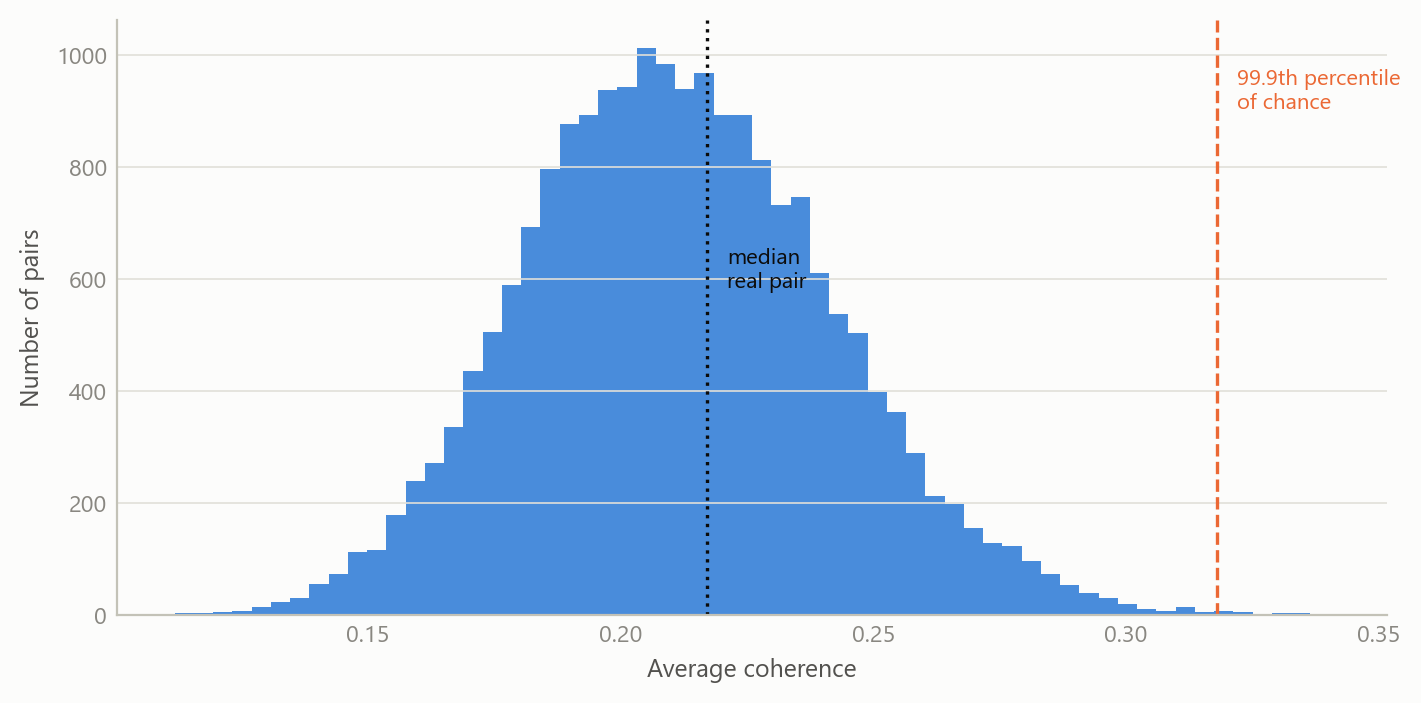
\includegraphics[keepaspectratio]{index_files/figure-latex/fig-null-output-1.png}}

}

\caption{\label{fig-null}Coherence between 20,000 pairs of independent
series passed through the screen's decomposition and coherence
estimator. The dashed line marks the 99.9th percentile of chance; the
dotted line the median pair of the real screen (simulated data).}

\end{figure}%

\textbf{But the excess over chance is large, and it sits where it
should.} By construction, one pair in a thousand clears the bar by
chance. Across the whole screen, more than one pair in twenty does. The
excess is concentrated: nearly half of all pairs of US energy price
series clear it, while pairs that mix Mexican and US series of other
kinds clear it only about once in a hundred.

\begin{figure}

\centering{

\pandocbounded{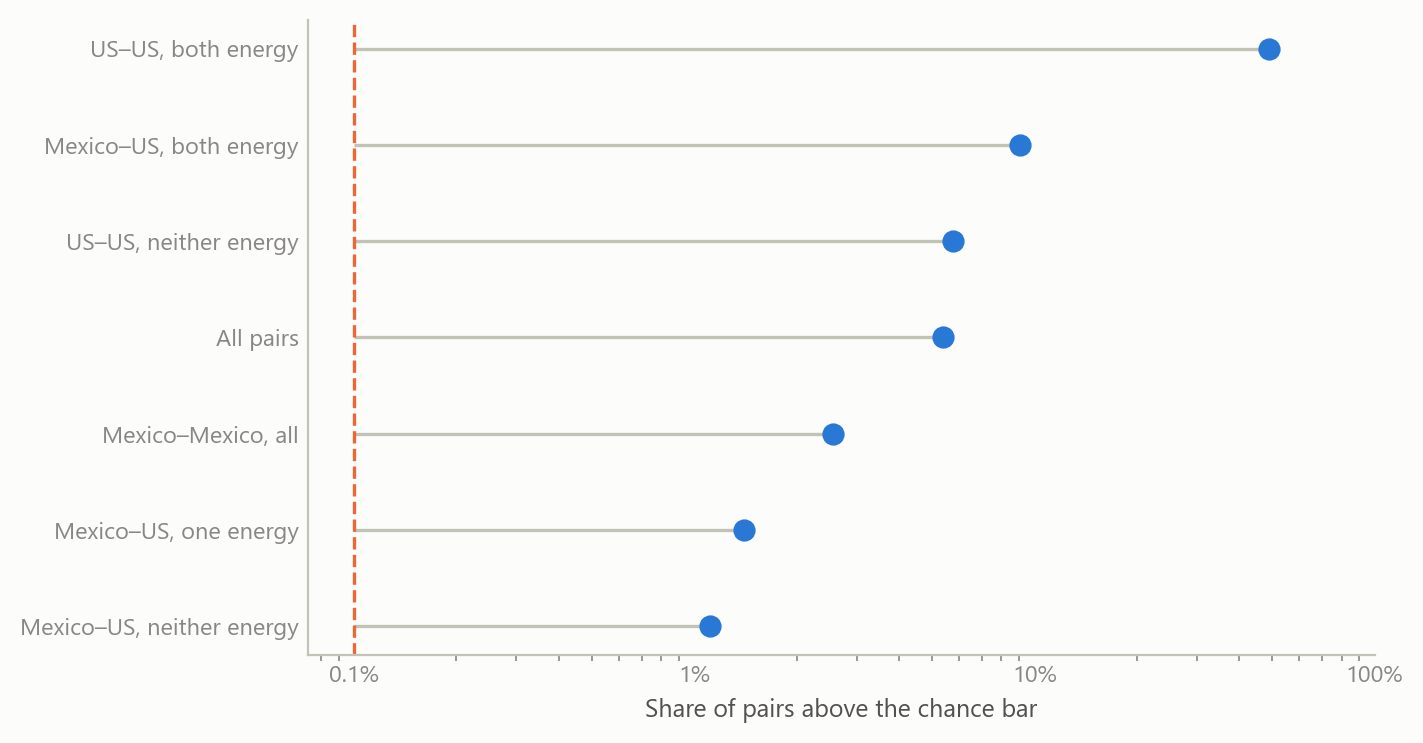
\includegraphics[keepaspectratio]{index_files/figure-latex/fig-groups-output-1.png}}

}

\caption{\label{fig-groups}Share of pairs whose coherence clears the
99.9th percentile of chance, by group of series, on a logarithmic scale.
The dashed line is the share expected by chance alone. Source: the
author's 2025 co-movement screen of monthly price and activity series;
chance benchmark simulated.}

\end{figure}%

The mixed Mexico--US groups also show the limits of a screen. Only 22
pairs in it link a Mexican and a US energy series, and they mix products
and measures: consumer against producer prices, city against region,
gasoline against electricity. A product-by-region comparison removes
that mix.

\begin{figure}

\centering{

\pandocbounded{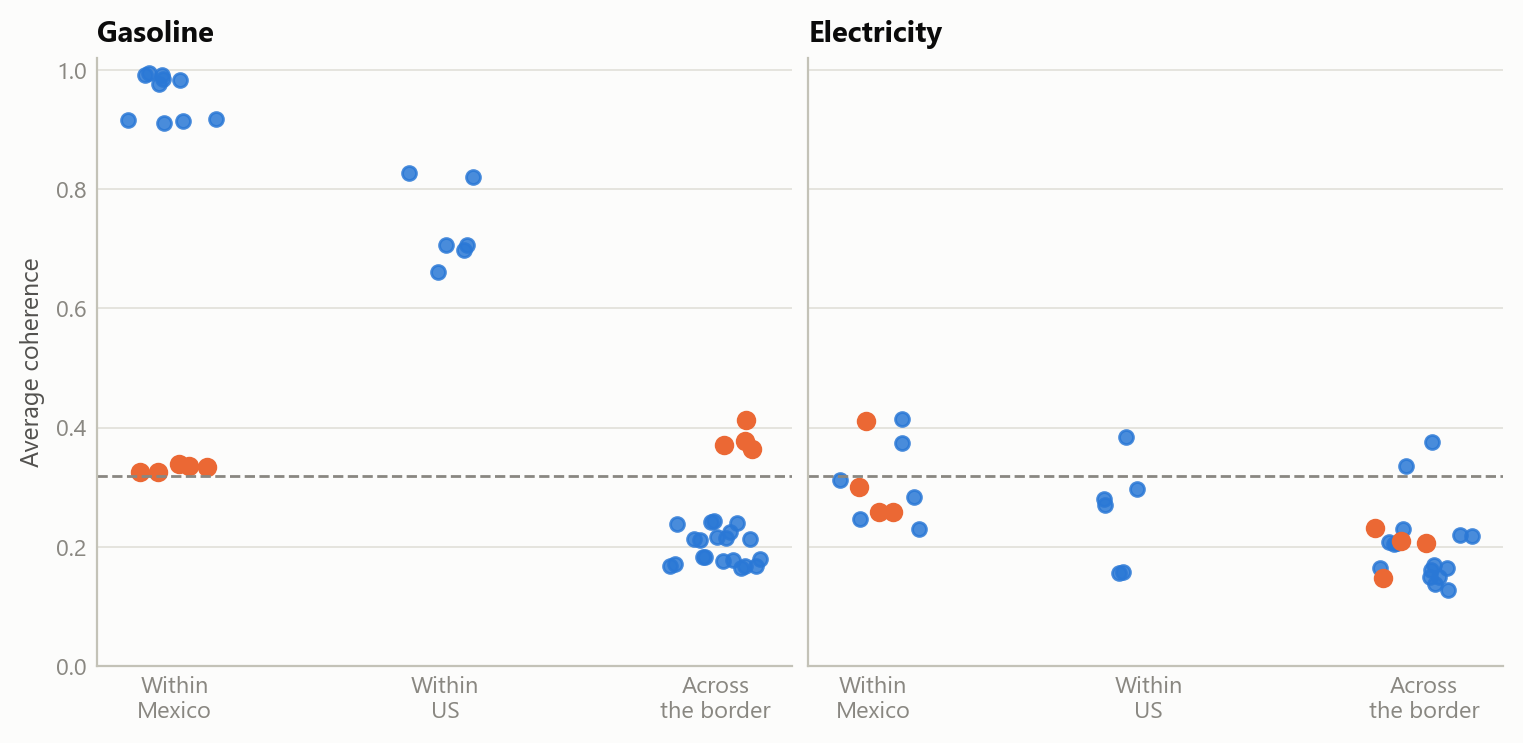
\includegraphics[keepaspectratio]{index_files/figure-latex/fig-pairs-output-1.png}}

}

\caption{\label{fig-pairs}Average coherence of the remainders for one
product across disjoint regions: within Mexico, within the United
States, and across the border. Orange points are pairs that involve
Mexico's northern border region. The dashed line is the 99.9th
percentile of chance. Source: the author's 2025 screen input, recomputed
in 2026; chance benchmark simulated.}

\end{figure}%

\textbf{Gasoline: integrated within each country, separate across the
border, except at the border.} Within Mexico, the median gasoline pair
has coherence 0.916 and every pair clears the bar. Within the United
States the median is 0.706, and again every pair clears it. Across the
border, the median falls to 0.213, around the level of chance. Only four
cross-border pairs clear the bar, and all four involve Mexico's northern
border region, one for each US census region (0.364 to 0.412). Each also
survives trimming and the time-shift test. The same region's five pairs
with other Mexican regions are the five lowest within Mexico (0.325 to
0.339), and none passes the time-shift test at the 1 per cent level.
Measured by the movement of its gasoline surprises, the northern border
region sits closer to the United States than to the rest of Mexico.

This is consistent with how fuel was priced there. For decades, gasoline
and diesel prices in Mexico were set by the government. A federal notice
for the first ten days of January 2017 set maximum gasoline prices for
the northern border region with fiscal stimuli set zone by zone,
including distance bands from the border running from 0--20 km to 40--45
km. Liberalisation then began in the border states of Baja California
and Sonora on 30 March 2017 and was scheduled to reach every remaining
state by 30 November 2017. Border prices set under their own rules would
let the region's surprises follow its neighbour's rather than the
national schedule. The data cannot confirm that mechanism; it can only
say the pattern is the one such a regime would produce.

\textbf{Electricity: no comparable pattern.} Within Mexico the median
electricity pair is 0.292, within the United States 0.275, and across
the border 0.206. Two of the 20 cross-border pairs clear the bar, both
linking Mexico's north-east to a US region (the Midwest, 0.376, and the
South, 0.336), and both pass the time-shift test. Two pairs out of 20
are a lead, not a pattern.

\textbf{One robust anomaly.} Of the screen's two Mexico--US energy pairs
above the bar, one, a US city's motor-fuel consumer price index against
Mexico's north-west gasoline index, has coherence 0.727. That holds at
0.695 after trimming and passes the time-shift test. It is far stronger
than any regional gasoline pair across the border, and nothing here
explains it. The other pair, a US producer price for industrial
electricity against Mexico's southern gasoline index (0.342), drops to
0.290 after trimming. That is below the bar, so a few extreme months
drive it.

\subsection{Insights}\label{insights}

\begin{itemize}
\tightlist
\item
  \textbf{A chance benchmark is the first output of a screen, not an
  afterthought.} For this estimator, unrelated series average about
  0.21, so a ranking that starts from zero overstates every pair. Once
  the bar is set by simulation, the question becomes where the excess
  sits, and that is informative.
\item
  \textbf{Holding the product fixed turns a ranking into a test.} The
  mixed cross-border group says only that a few pairs stand out. The
  same product in disjoint regions says which regions are integrated and
  which are not.
\item
  \textbf{The border shows up as a region, not as a product.} Gasoline
  is integrated within each country. The one cross-border link runs
  through a single Mexican region, and the same region is the least
  connected to the rest of Mexico.
\item
  \textbf{Robustness checks separate leads from artefacts.} Trimming
  removed one of the screen's two cross-border energy pairs. The
  time-shift test sorted the regional pairs into those that hold at the
  true alignment and those that do not.
\end{itemize}

\subsection{Limits and next steps}\label{limits-and-next-steps}

Coherence averaged over all frequencies says that two surprise series
move together, not which leads, by how much, or at what horizon. The
natural next step is to report phase and gain by frequency band for the
four northern-border pairs. Splitting the sample at 2017 would then test
whether the border region's link to the United States changed with
liberalisation, which would turn the policy reading from ``consistent
with'' into a test.

The policy timeline is context, not evidence: the analysis does not
observe border fuel prices directly. The composition of Mexico's
statistical regions is not used, so the reading by state is indicative
only. Regional consumer price sub-indices are noisy, and the estimator's
floor of about 0.21 limits what modest coherence can show.

The robust anomaly, a single US city's motor-fuel index moving closely
with Mexico's north-west gasoline index, is the open lead. It needs
checking against how the two series are constructed before any economic
reading. Until then it is reported, not interpreted.

\subsection{About the evidence}\label{about-the-evidence}

The screen ran in 2025 over a licensed commercial database of price and
activity series. Its input is not reproduced here, and series are
described by category only. The chance benchmark, the product-by-region
comparison, the trimming and the time-shift tests were computed in 2026
from the screen's own input, with an exact replica of its estimator that
matches its stored values to rounding error. The first figure is
simulated. The second and third plot statistics derived from the real
series. The policy dates come from a 2017 industry report on Mexico's
fuel-price liberalisation and from the text of the January 2017 federal
notice.

Figures and tables marked \emph{simulated} are generated from simulated
data built to share the structure of the analysis (its variables,
horizons and frequencies). They show how the method works and what its
output looks like; they are not the project's results. Results stated in
the text are the project's own. Methods are described at the level of a
methods section. Code and data pipelines are not reproduced here.




\end{document}
